\chapter{Datenerfassung und -aufbereitung}

\section{Beschreibung der gesammelten Daten}
\begin{itemize}
    \item \textbf{Datenerhebungsmethoden:} Erklären Sie, wie die Daten gesammelt wurden (z.B. welche Geräte, Orte und Zeitpunkte).
    \item \textbf{Datensätze und Umfang:} Beschreiben Sie den Umfang und die Struktur der gesammelten Datensätze.
    \item \textbf{Datenqualität und -validität:} Diskutieren Sie die Qualität und Validität der Daten.
\end{itemize}

Es wurden insgesamt 407 Messungen in 35 Räumen durchgeführt. Die Messungen wurden zwischen dem 8. Mai 2024 und dem 31. Mai 2024 durchgeführt. Im Schnitt wurden bei jeder Messung 12,8 Router erfasst. Im Schnitt wurden 11,6 Messungen pro Raum durchgeführt. Die Anzahl der Messungen pro Raum variiert zwischen 2 und 19. Es wurden insgesamt 318 Router erfasst.

Die Anzahl der Messungen pro Raum sind in Abbildung \ref{fig:0_general_01} dargestellt.

\begin{figure}[H]
    \centering
    \includegraphics[width=0.8\textwidth]{images/0_general_01.png}
    \caption{Beispielabbildung 1}
    \label{fig:0_general_01}
\end{figure}

\begin{itemize}
    \item Verwendete Geräte (Doogee Y8, Google Pixel 8, Samsung Galaxy A?!)
\end{itemize}

\section{Vorbereitungsprozesse}
\begin{itemize}
    \item \textbf{Datenbereinigung:} Erklären Sie, wie die Daten bereinigt und aufbereitet wurden.
    \item \textbf{Feature-Engineering:} Beschreiben Sie die durchgeführten Schritte zur Erstellung und Auswahl von Features.
    \item \textbf{Datenaufteilung:} Diskutieren Sie die Aufteilung der Daten in Trainings- und Testsets.
\end{itemize}

\section{Erste Parameteroptimierung}
\begin{itemize}
    \item \textbf{Parameterraum:} Beschreiben Sie den Parameterraum, der in der ersten Optimierungsrunde untersucht wurde.
    \item \textbf{Optimierungsverfahren:} Erklären Sie das Verfahren zur Auswahl der besten Parameter (z.B. Grid Search, Cross-Validation).
    \item \textbf{Ergebnisse und Auswahl:} Diskutieren Sie die Ergebnisse der Optimierung und die Auswahl der besten Parameter.
\end{itemize}

TODO: Es muss auch irgendwo stehen was der average und der weighted average ist und warum beides in den Plots gezeigt qwird!

Die besten Parameter für die Algorithmen sind in den Abbildungen \ref{fig:2_best_parameters_01} und \ref{fig:2_best_parameters_02} dargestellt.

Warum diese Parameter?
\begin{itemize}
    \item KNN: 1, 3, 5, 7, 9, 11, 13, 15 -> 
    \item RF: 50, 100, 150, 200, 250, 300, 350, 400 Wurde gewählt, weil 407 Messpunkte existieren
    \item SVM: 0.001, 0.005, 0.01, 0.05, 0.1, 0.5, 1, 5 -> Quelle: Supervised Learning-Based Indoor Positioning System Using WiFi Fingerprints Seite 62
\end{itemize}    

Ergebnisse:

\begin{itemize}
    \item KNN: 5, 7, 9 
    \item RF: 100, 200, 300
    \item SVM (RBF): 0.5, 1, 5
    \item SVM (Linear): 0.001, 0.005, 0.01
\end{itemize}   

\paragraph{KNN}
% \linebreak

Bei der KNN-Analyse wurden die Werte 5, 7 und 9 für k ausgewählt. Wie in Abbildung \ref{fig:2_best_parameters_01} zu sehen ist, zeigen die Genauigkeiten, dass bei Räumen mit wenigen Messungen kleinere k-Werte bessere Ergebnisse liefern, während bei Räumen mit mehr Messungen größere k-Werte vorteilhafter sind. Diese Tendenz ist sowohl bei der euclidean- als auch bei der sorensen-Metrik zu beobachten.


Abbildung \ref{fig:2_best_parameters_02} zeigt, dass bei average/euclidean die Werte 3, 5 und 7 die besten Ergebnisse liefern, während bei weighted average/euclidean die Werte 5, 7 und 9 am besten abschneiden. Bei average/sorensen erzielen die Werte 5, 7 und 9 die besten Ergebnisse, und bei weighted average/sorensen sind es die Werte 5, 7 und 13, wobei die Genauigkeit bei k = 9 und k = 11 kaum von der Genauigkeit bei k = 13 abweicht.

Generell ist die Genauigkeit bei mehreren Messungen pro Raum weniger stark von k abhängig als bei wenigen Messungen pro Raum, mit Ausnahme von sehr kleinen k-Werten wie 1 oder 3. Daher wurden für die weiteren Analysen die k-Werte 5, 7 und 9 gewählt.

\paragraph{Random Forest}
% \linebreak

Wie in Abbildung \ref{fig:2_best_parameters_01} zu sehen ist, hat der Wert für n\_estimators beim Random-Forest-Algorithmus keinen großen Einfluss. Aus diesem Grund wurden die Werte 100, 300 und 500 gewählt, um eine gleichmäßige Verteilung zu gewährleisten.

\paragraph{SVM (linear)}
% \linebreak


Interessanterweise wurden bei der linearen SVM unabhängig vom Parameter C alle Räume korrekt vorhergesagt. Sollte man vielleicht in Betracht ziehen, alle Räume mit nur 5 Messungen zu verwenden und den SVM-Algorithmus anzuwenden? Die Ursache könnte Zufall sein (weniger Messungen führen zu größerer Streuung) oder der Algorithmus ist tatsächlich so gut. Ansonsten nimmt die Genauigkeit mit zunehmendem Wert für C ab. Die besten Werte bei average und weighted average wurden für die Werte 0,001, 0,005 und 0,01 erzielt. Daher wurden für die weitere Analyse die Werte C = 0.001, 0.005 und 0.01 gewählt.

\paragraph{SVM (rbf)}
% \linebreak

Generell lässt sich in Abbildung \ref{fig:2_best_parameters_01} erkennen, dass größere Werte für C bessere Ergebnisse liefern als kleinere. Die besten Ergebnisse konnten bei average und weighted average für C = 1.0 erzielt werden. Daher wurden für die weitere Analyse die Werte C = 0.5, 1.0 und 5.0 gewählt.

% Brauch ich das noch? zeigen die Genauigkeiten, dass bei Räumen mit wenigen Messungen kleinere n\_estimators-Werte bessere Ergebnisse liefern, während bei Räumen mit mehr Messungen größere n\_estimators-Werte vorteilhafter sind. Diese Tendenz ist sowohl bei der euclidean- als auch bei der sorensen-Metrik zu beobachten. Abbildung \ref{fig:2_best_parameters_02} zeigt, dass bei average

\begin{figure}[H]
    \centering
    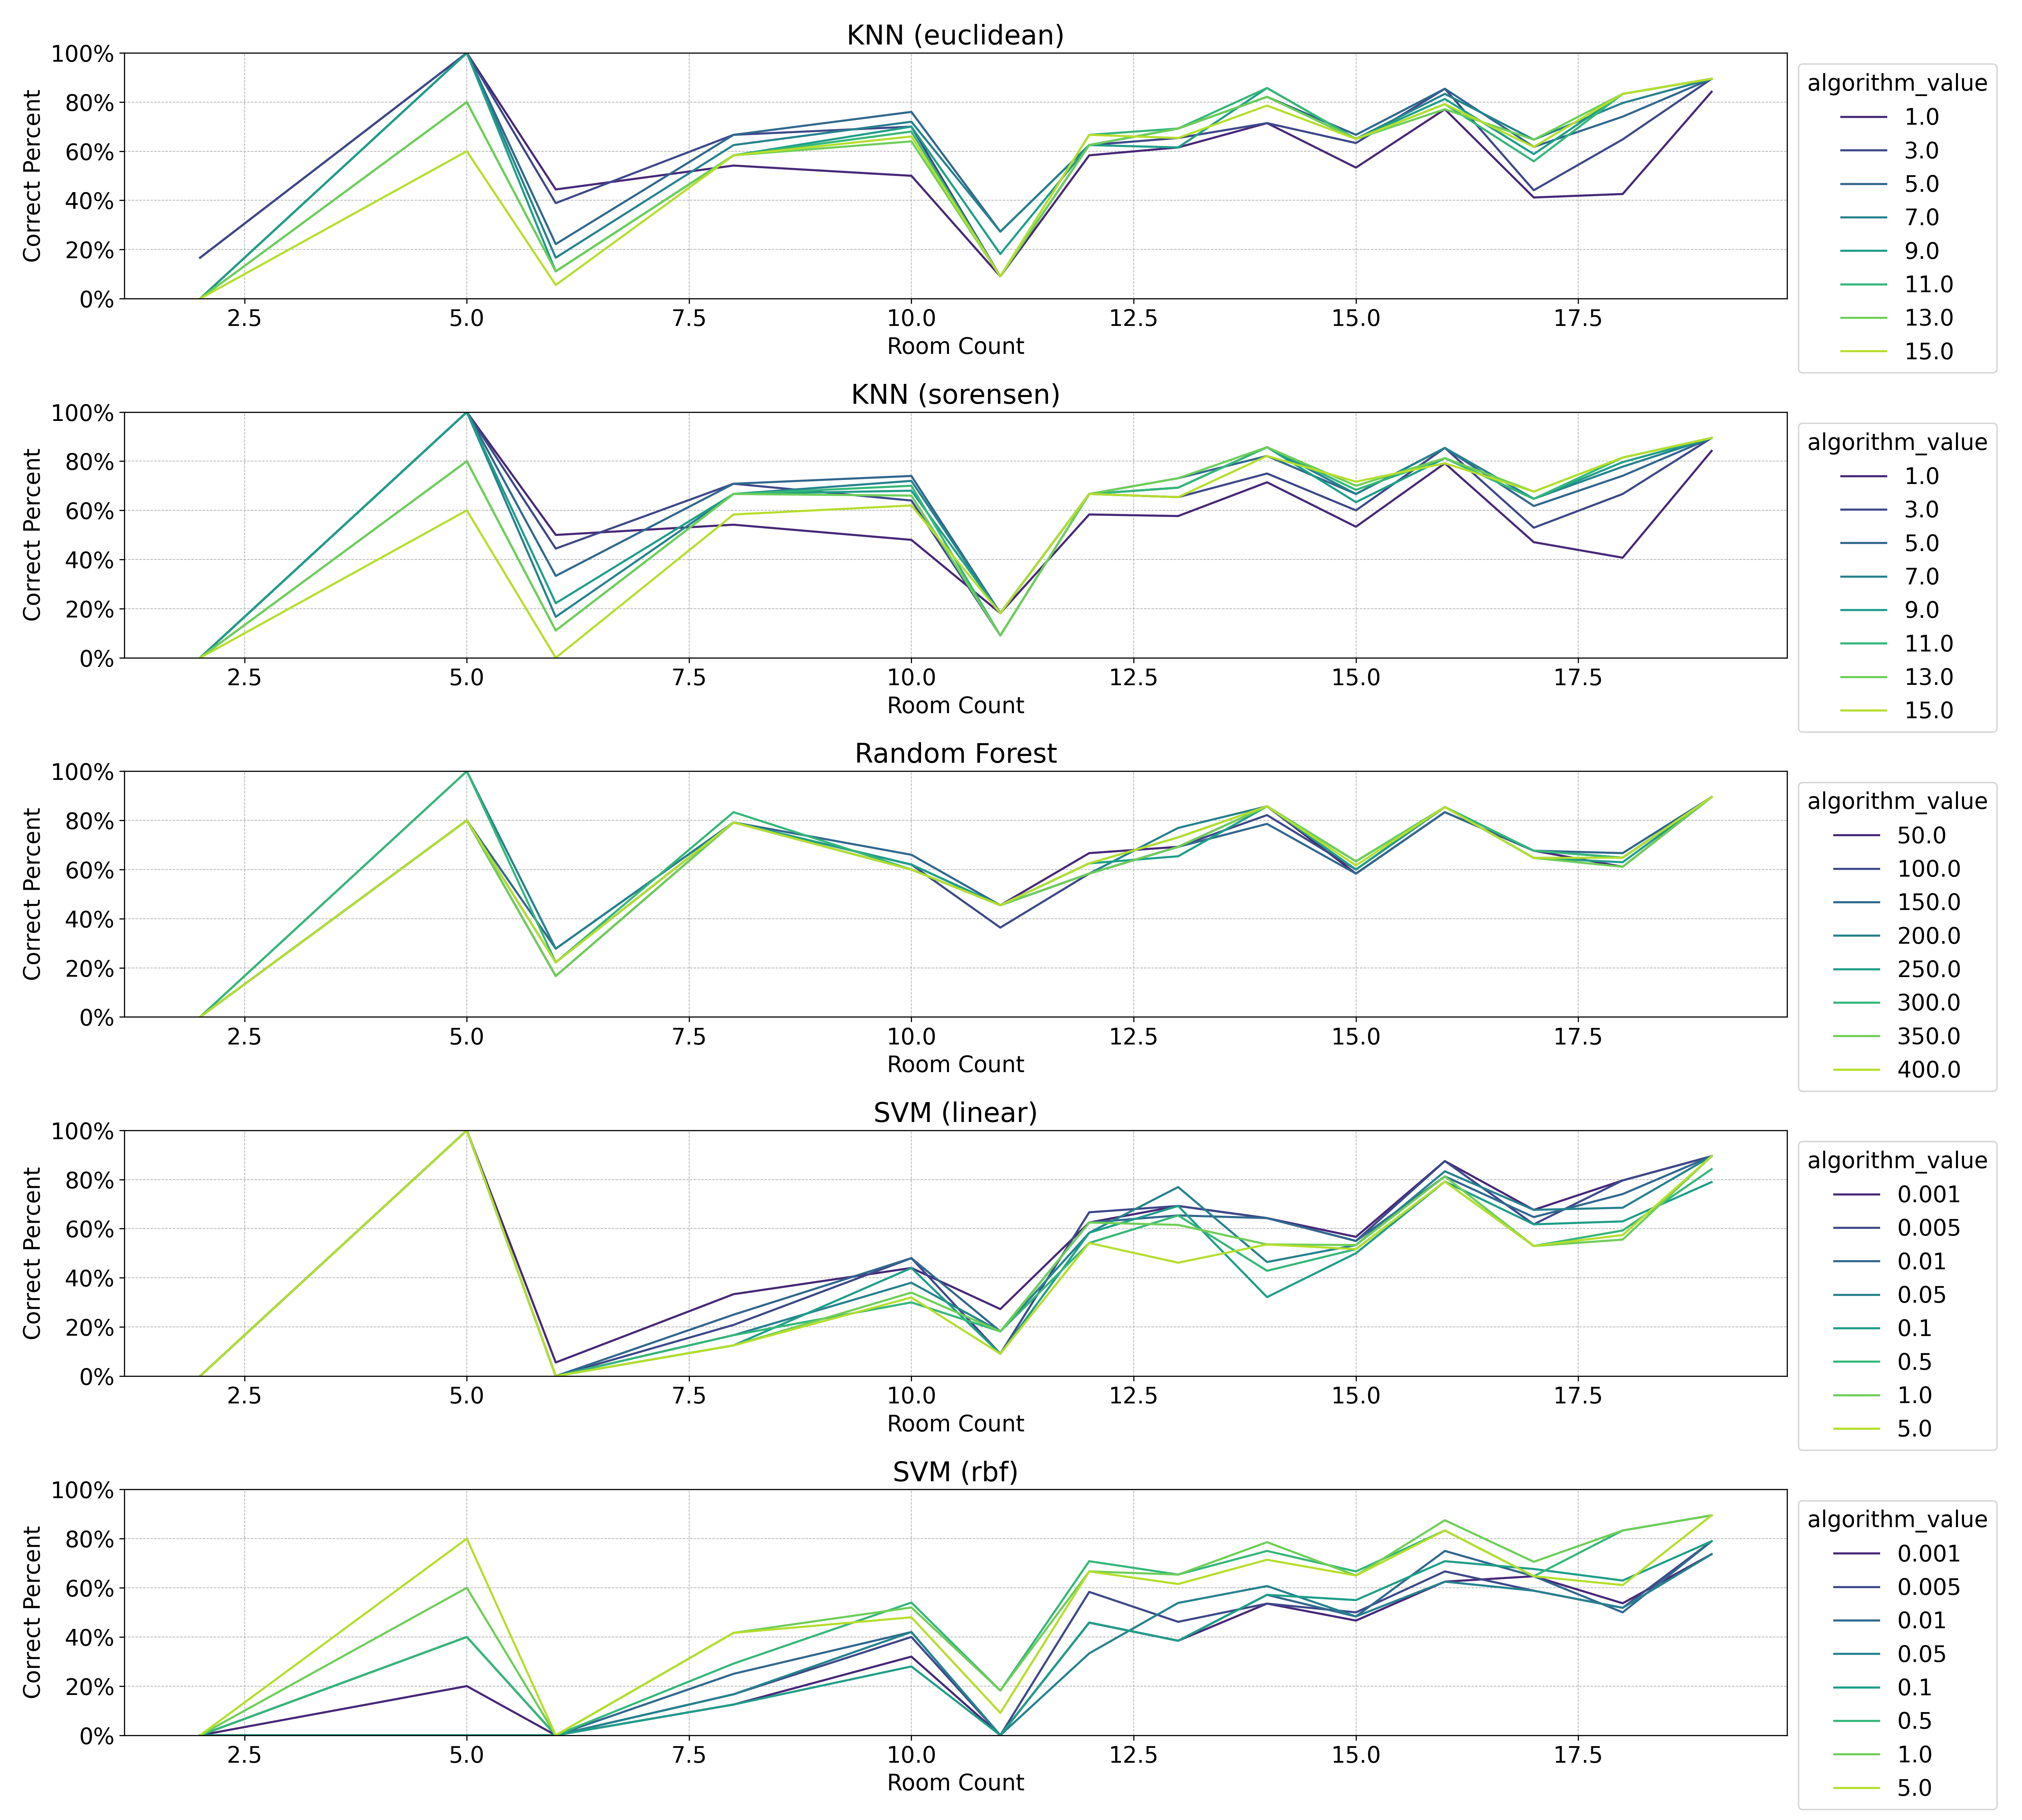
\includegraphics[width=0.8\textwidth]{images/2_best_parameters_01.png}
    \caption{Auswahl der Parameter}
    \label{fig:2_best_parameters_01}
\end{figure}

\begin{figure}[H]
    \centering
    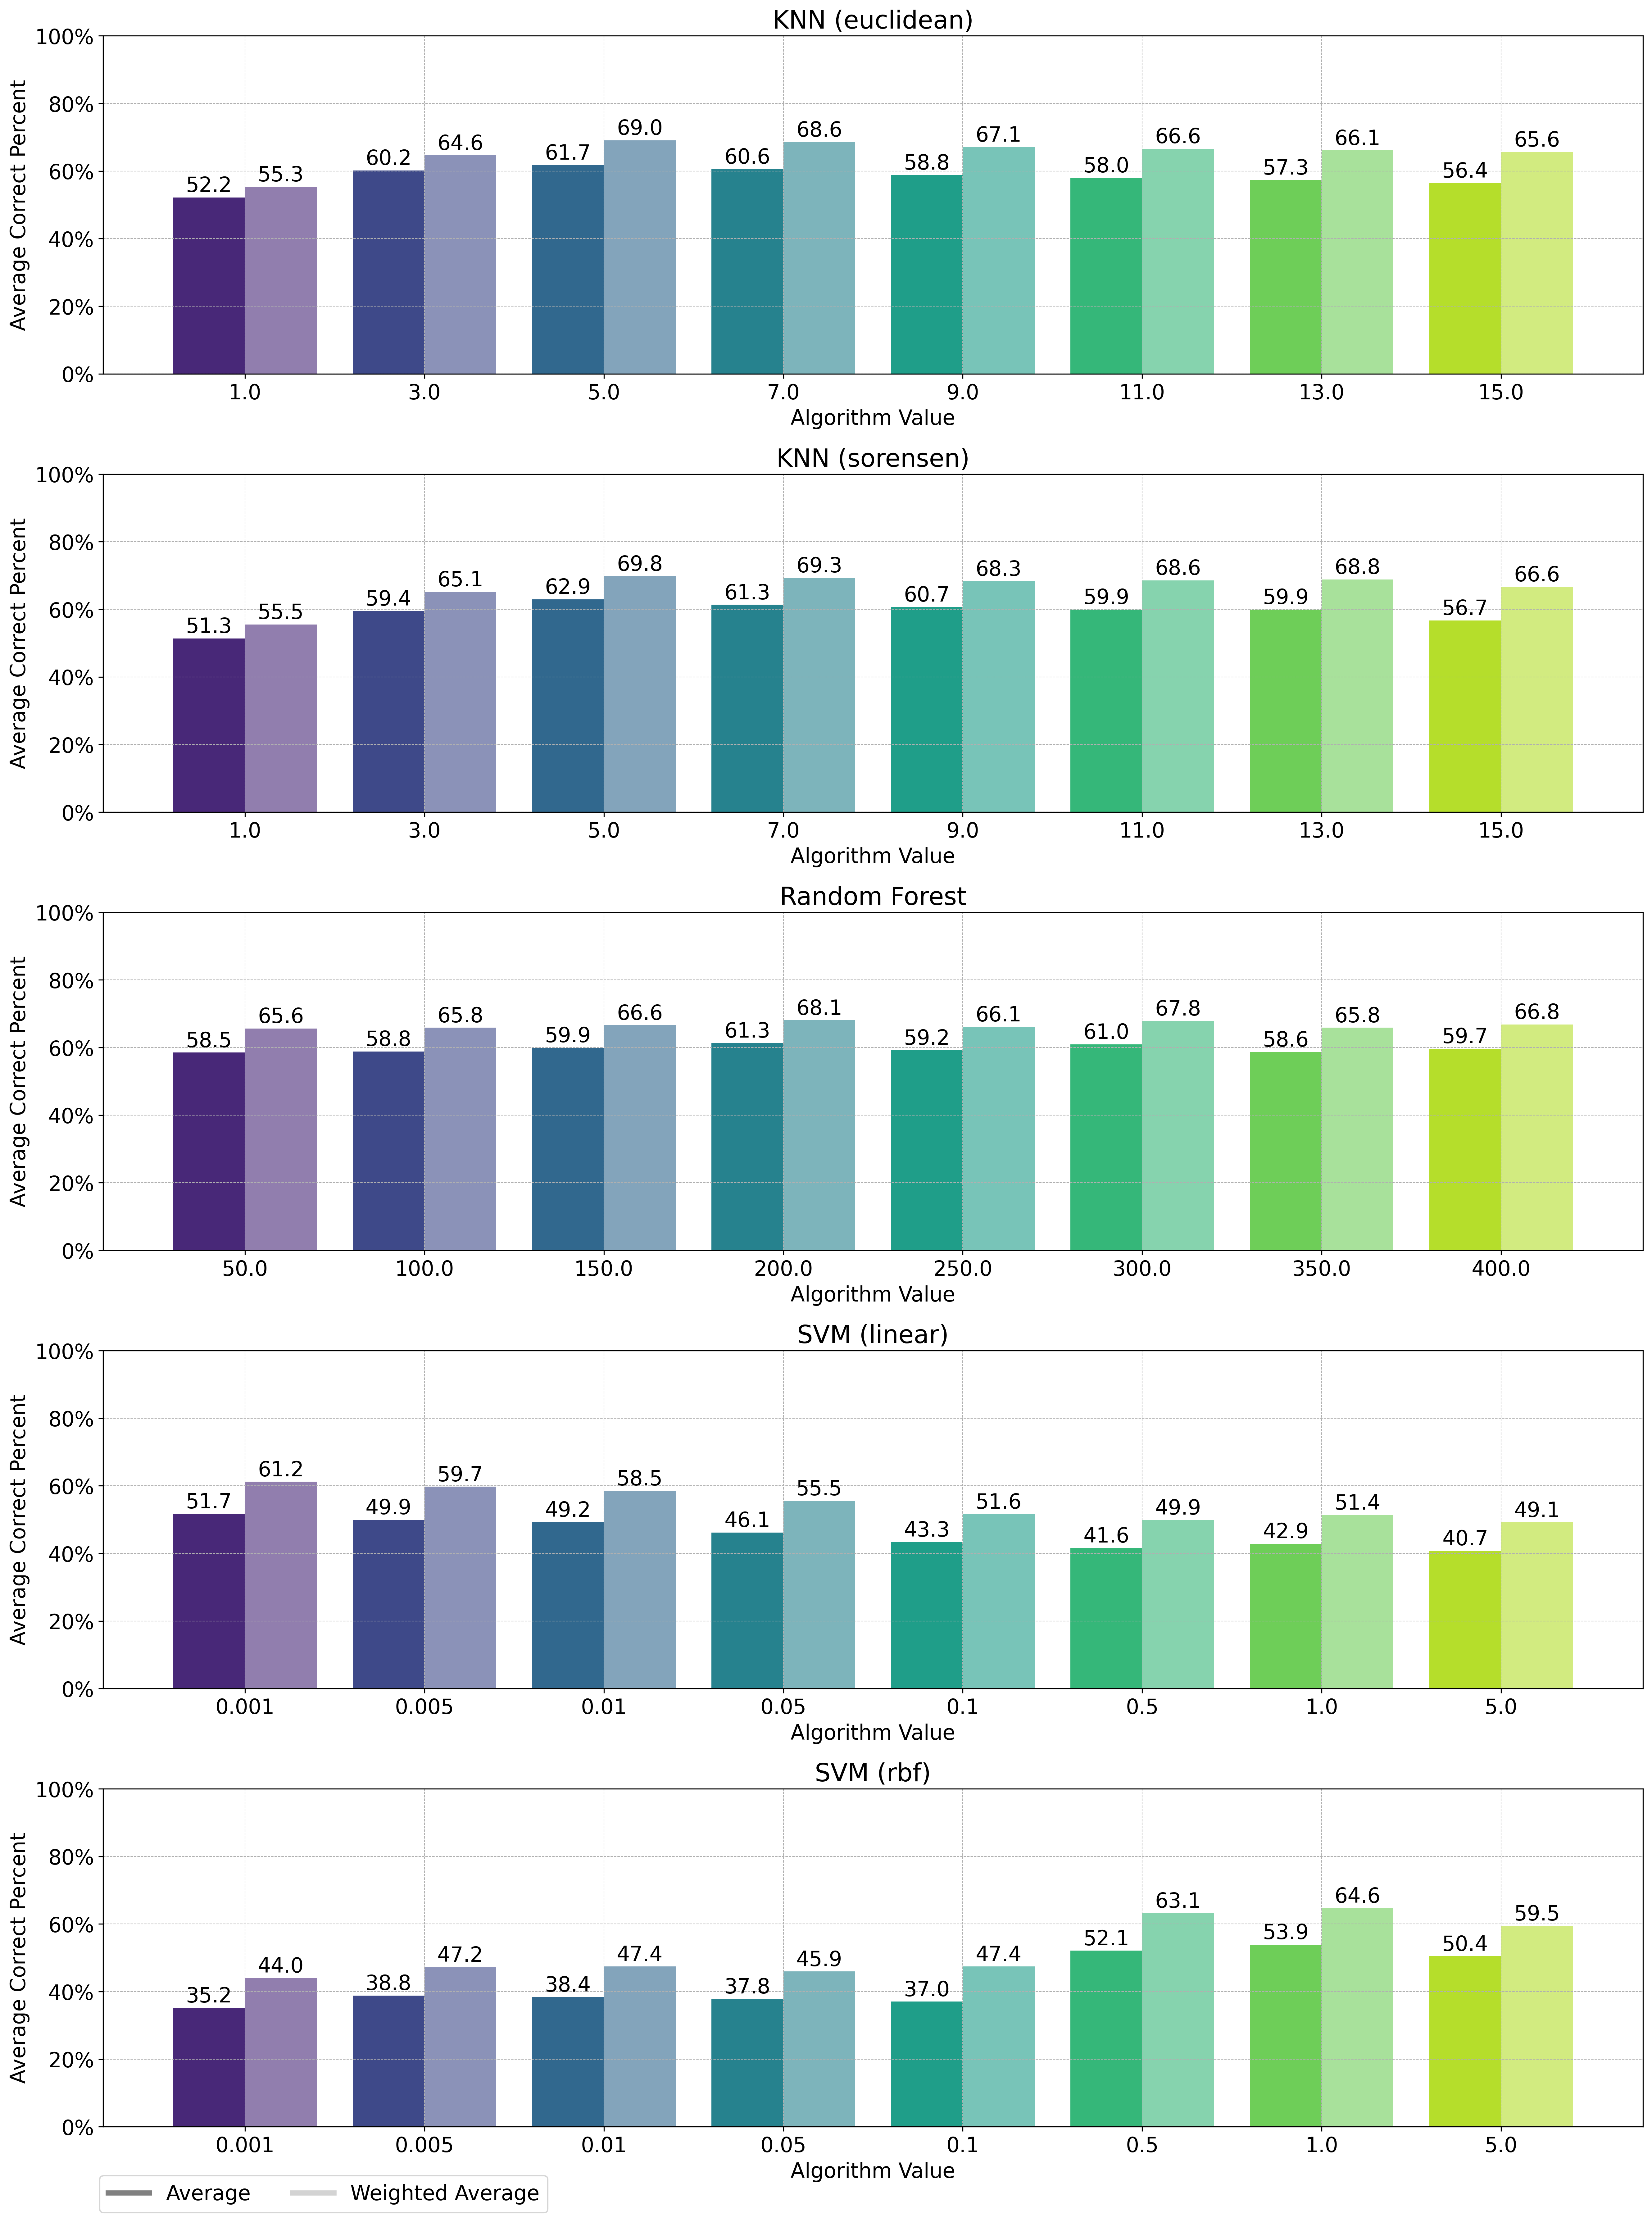
\includegraphics[width=0.8\textwidth]{images/2_best_parameters_02.png}
    \caption{Auswahl der Parameter}
    \label{fig:2_best_parameters_02}
\end{figure}

\section{Strategien für den Umgang mit fehlenden Werten}
\begin{itemize}
    \item \textbf{Fehlende Werte identifizieren:} Erklären Sie, wie fehlende Werte in den Daten identifiziert werden.
    \item \textbf{Umgangsstrategien:} Beschreiben Sie verschiedene Strategien zum Umgang mit fehlenden Werten (z.B. Imputation, Ignorieren).
    \item \textbf{Vergleich der Strategien:} Diskutieren Sie die Vor- und Nachteile der verschiedenen Strategien und deren Einfluss auf die Ergebnisse.
\end{itemize}

Die Ergebnisse der verschiedenen Strategien zur Behandlung fehlender Werte sind in Abbildung \ref{fig:3_handle_missing_values_strategy_01} dargestellt.

\begin{itemize}
    \item use\_received ist am schlechtesten, -100 ist am besten und zero ist nur etwas schlechter als -100
    \item das beste ergebnis war bei knn/sorensen/k=5 mit 62,2 \% 
    \item -100 und zero haben einen sehr ähnlichen Verlauf, wobei dieser bei RF fast identisch ist und bei den anderen leicht verschieden
    \item use\_received ist bei RF und KNN schlecht und folgt auch nicht dem gleichen Verlauf wie die anderen. bei SVM folgt es dem Verlauf von -100 und zero
\end{itemize}

\begin{figure}[H]
    \centering
    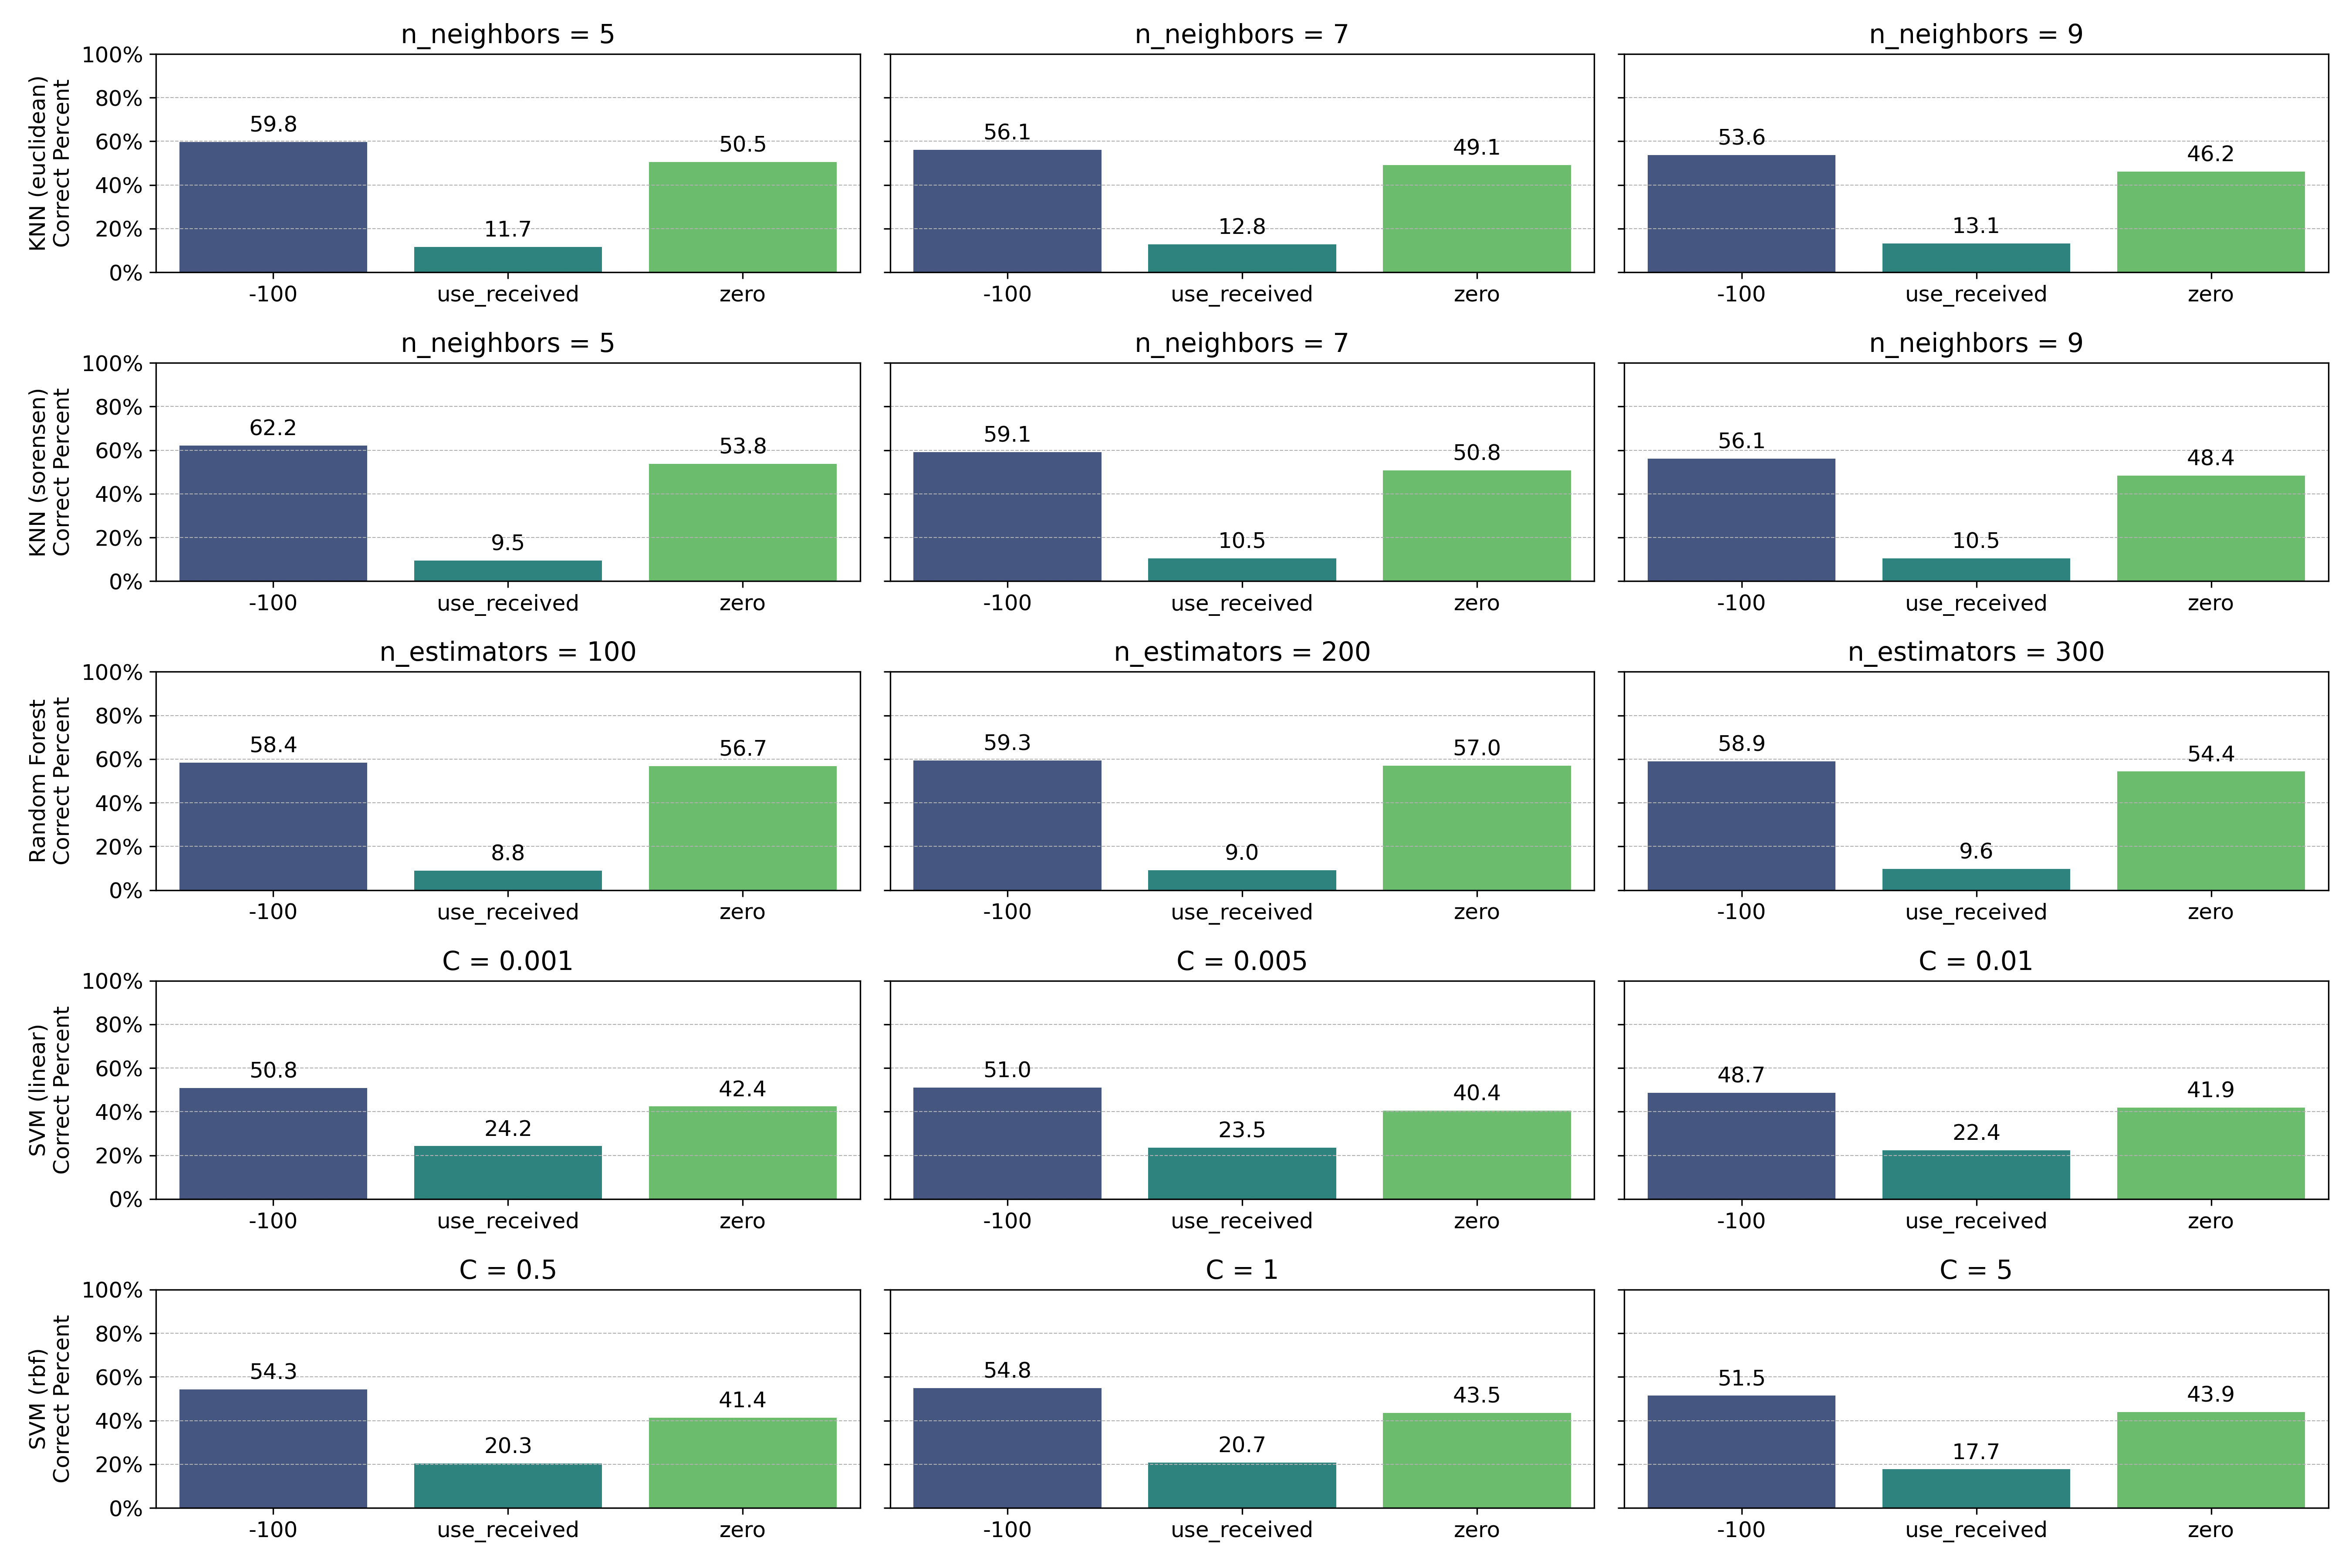
\includegraphics[width=0.8\textwidth]{images/3_handle_missing_values_strategy_01.png}
    \caption{Fehlende Werte}
    \label{fig:3_handle_missing_values_strategy_01}
\end{figure}

\section{Auswahl der zu verwendenden Router}
\begin{itemize}
    \item \textbf{Kriterien für die Auswahl:} Erklären Sie die Kriterien, nach denen Router für die Analyse ausgewählt werden.
    \item \textbf{Unterschiedliche Router-Sets:} Beschreiben Sie die verschiedenen Router-Sets (z.B. alle Router vs. nur Eduroam).
    \item \textbf{Einfluss der Auswahl:} Diskutieren Sie den Einfluss der Router-Auswahl auf die Ergebnisse.
\end{itemize}

Die Ergebnisse der verschiedenen Strategien zur Auswahl der Router sind in Abbildung \ref{fig:4_router_selection_01} dargestellt.

\begin{itemize}
    \item Alle Router sind besser als nur die eduroam Router
    \item Unterschiede nehmen mit zunehmener Anzaahl der Messungen eines Raums ab.
    \item Es wird sich trotzdem für alle Router entschieden, da die Unterschiede hauptsächlich bei wenigen Messungen auftreten und dort eine größere Streuung erwaret wird und bei den eduroam Routern sichergestellt werden kann, dass diese nicht die Position verändern 
\end{itemize}    

\begin{figure}[H]
    \centering
    \includegraphics[width=0.8\textwidth]{images/4_router_selection_01.png}
    \caption{Auswahl der Router}
    \label{fig:4_router_selection_01}
\end{figure}

\section{Schwellenwert für Routerpräsenz}
\begin{itemize}
    \item \textbf{Filterkriterien:} Beschreiben Sie die Kriterien, nach denen Messwerte gefiltert werden (z.B. Signalstärke).
    \item \textbf{Filtermethoden:} Erklären Sie die angewendeten Filtermethoden und deren Implementierung.
    \item \textbf{Vergleich der Methoden:} Diskutieren Sie die Ergebnisse der Filterung und deren Einfluss auf die Datenqualität.
\end{itemize}

Die Ergebnisse der verschiedenen Strategien zur Auswahl des Router Presence Threshold sind in Abbildung \ref{fig:5_router_presence_threshold_01} dargestellt.

\begin{itemize}
    \item Router die in mehreren Messungen eines Raums vorhanden sind, sind aussagekräftiger als Router die nur in wenigen Messungen vorhanden sind
    \item Also: In wie viel Prozent der Messungen muss ein Router vorhanden sein, damit er berücksichtigt wird
    \item Das bedeutet, dass bei wenig Messungen die Auswirkungen gering sein sollten
\end{itemize}    

\begin{itemize}
    \item bei allen Algorithmen ist 0 am besten
    \item Interessant: Bei allen Algos haben die Genauigkeiten in Abhängigkkeit der Messungen pro Raum einen ähnlichen Verlauf und sind mit zunehmendem Router Presence Threshold schlechter, AUSSER bei SVM. Doer sind bei wenigen Messungen die größeren Router Presence Thresholds besser und bei mehr Messungen die kleineren. -> Deswegen wurde hier 0.25 verwendet, da dieser Wert im Schnitt die besten Ergebnisse erzielt
    \item SVM-Kipppunkt bei 10
\end{itemize}

\begin{figure}[H]
    \centering
    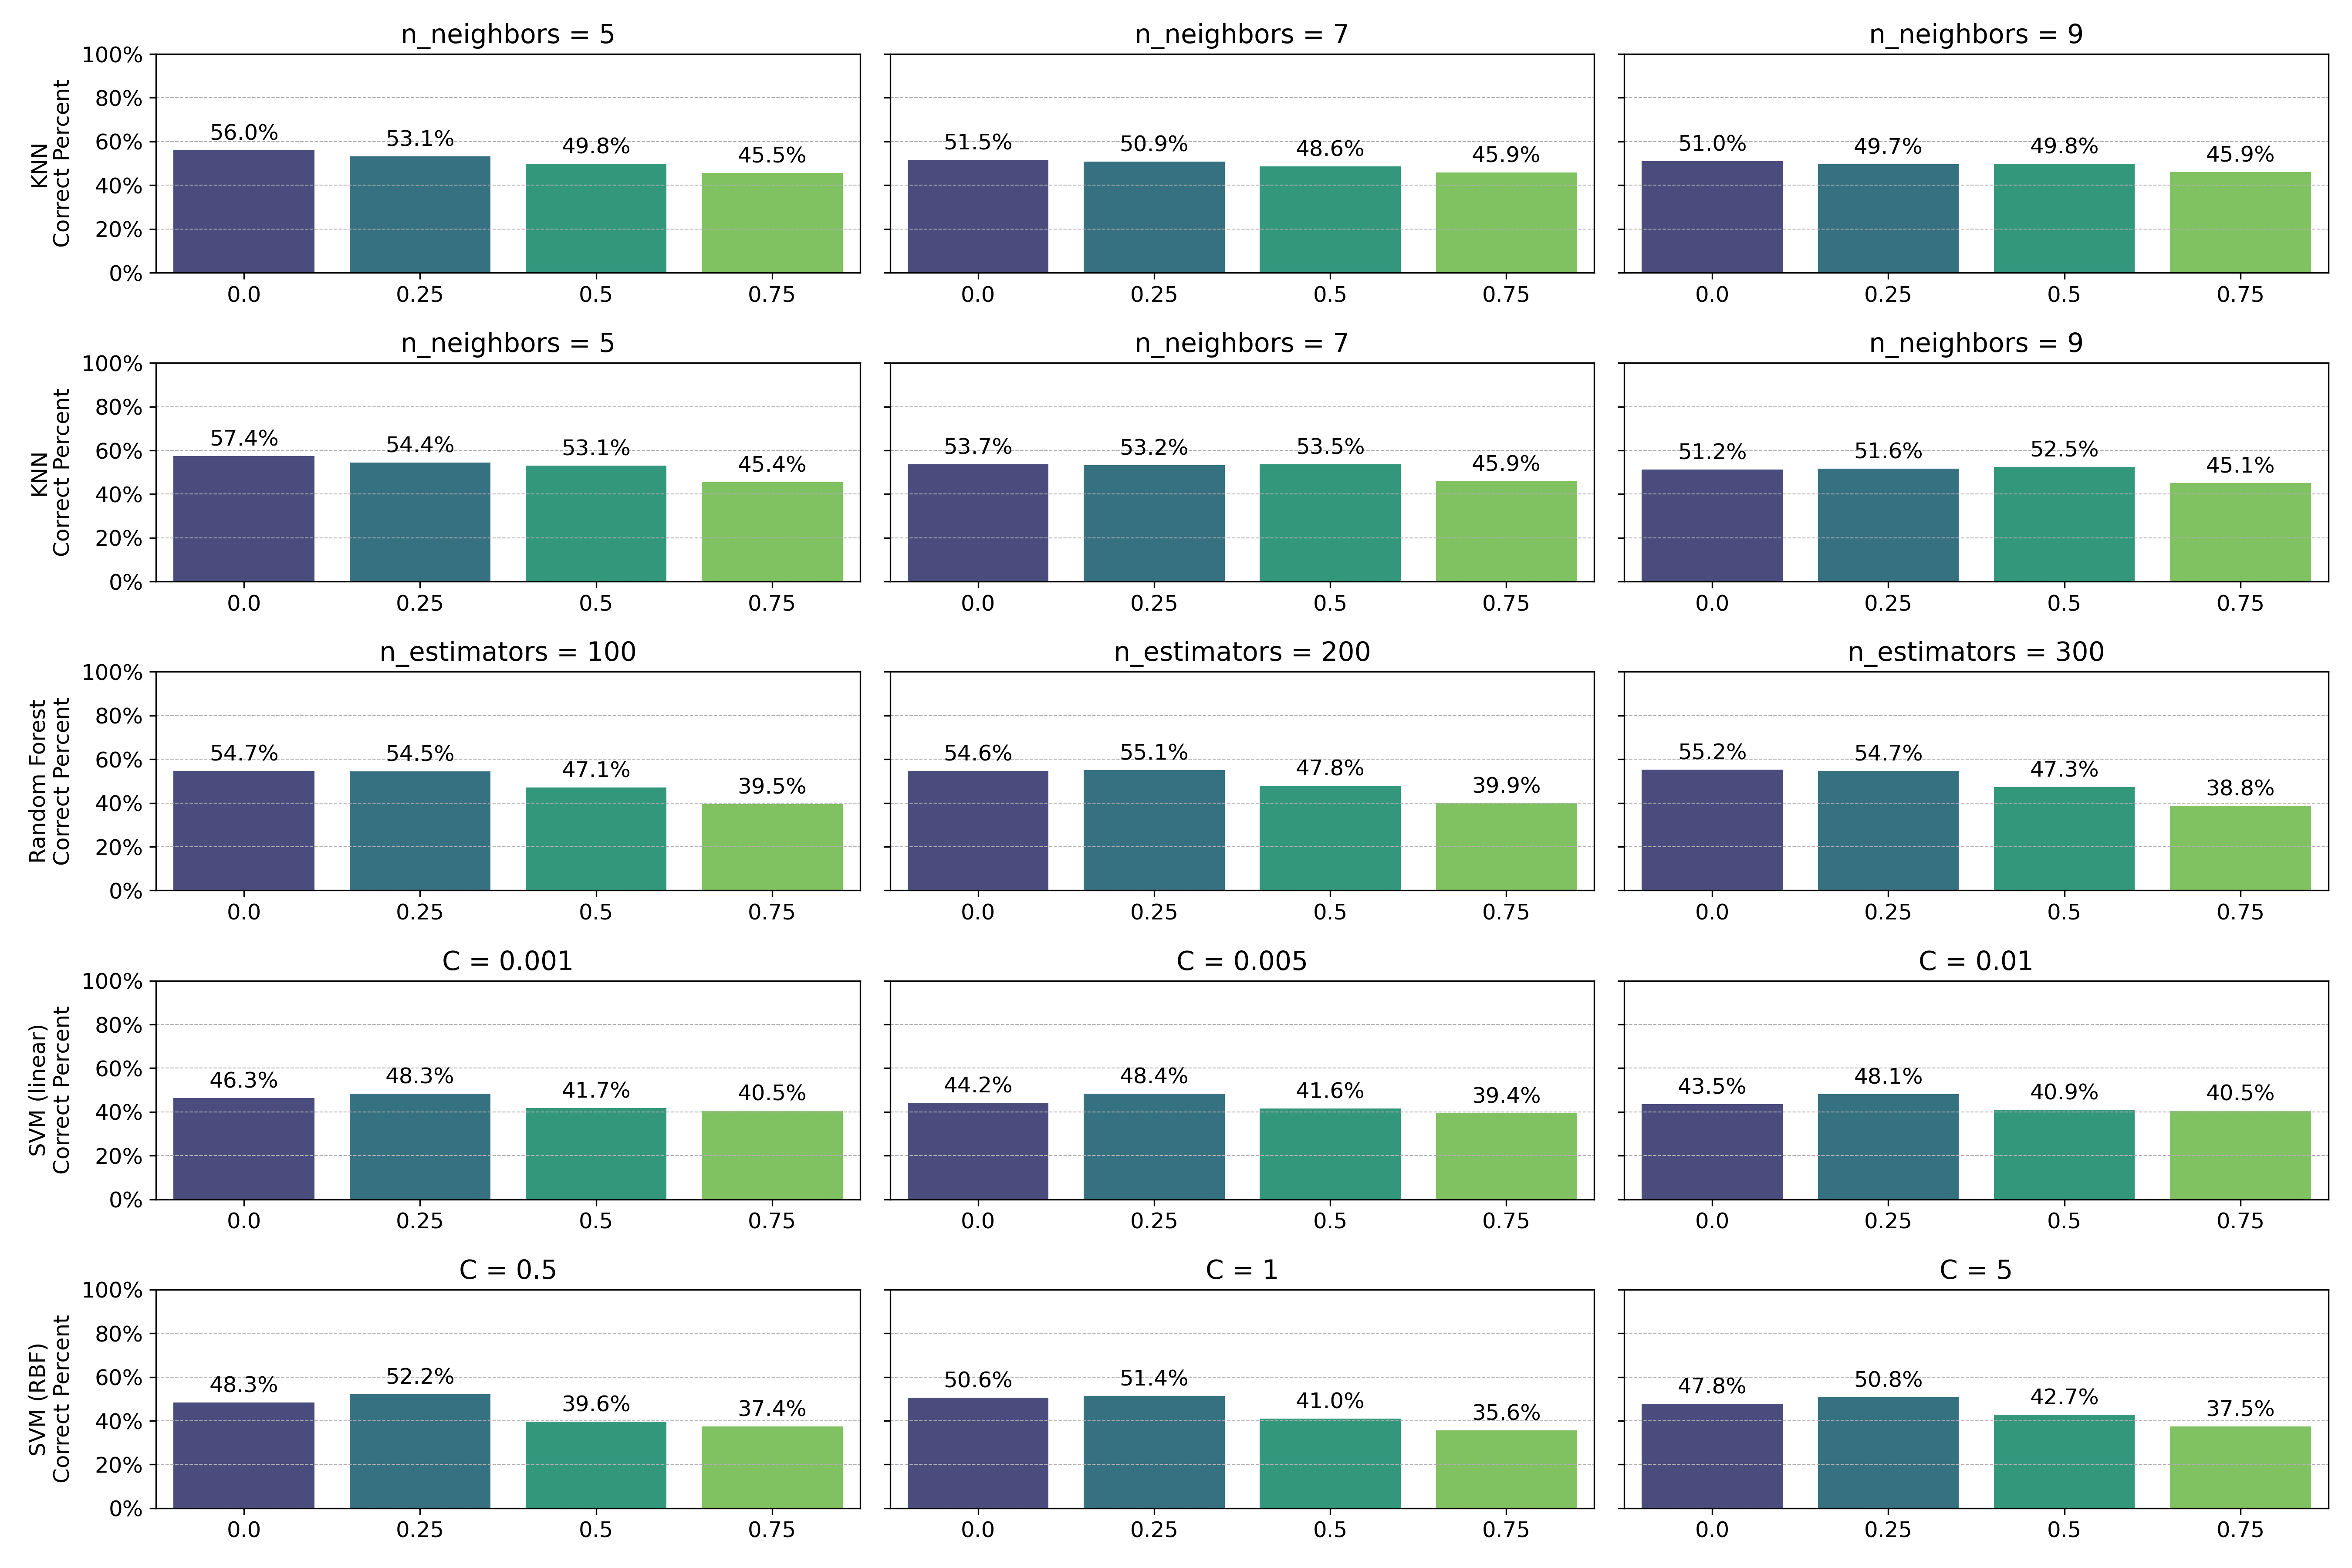
\includegraphics[width=0.8\textwidth]{images/5_router_presence_threshold_01.png}
    \caption{Router Presence Threshold}
    \label{fig:5_router_presence_threshold_01}
\end{figure}

\section{Schwellenwert für Router-RSSI}
\begin{itemize}
    \item \textbf{Filterkriterien:} Beschreiben Sie die Kriterien, nach denen Messwerte gefiltert werden (z.B. Signalstärke).
    \item \textbf{Filtermethoden:} Erklären Sie die angewendeten Filtermethoden und deren Implementierung.
    \item \textbf{Vergleich der Methoden:} Diskutieren Sie die Ergebnisse der Filterung und deren Einfluss auf die Datenqualität.
\end{itemize}

Die Ergebnisse der verschiedenen Strategien zur Auswahl des Router Rssi Threshold sind in Abbildung \ref{fig:6_router_rssi_threshold_01} dargestellt.

\begin{itemize}
    \item Idee: sehr kleine RSSI Werte werden ignoriert/so getan, als wäre die bei der Messung nicht dabei
    \item Gedanke dahiner: Router mit größeren RSSI-Werten sind aussagekräftiger und sollten dadurch mehr Einfluss haben
    \item Ergebnis: Bei allen Algorithmen ist -100 am besten -> Router mit geringen RSSI-Werten haben einen größeren Einfluss als vermutet
    \item Idee ist nicht von mir, sondern kommt aus dem Paper: Quelle: Comprehensive analysis of distance and similarity measures for Wi-Fi fingerprinting indoor positioning systems
    \item Die Thresholds sind: -100, -90, -80, -70, -60, -50, -40
\end{itemize}    

\begin{figure}[H]
    \centering
    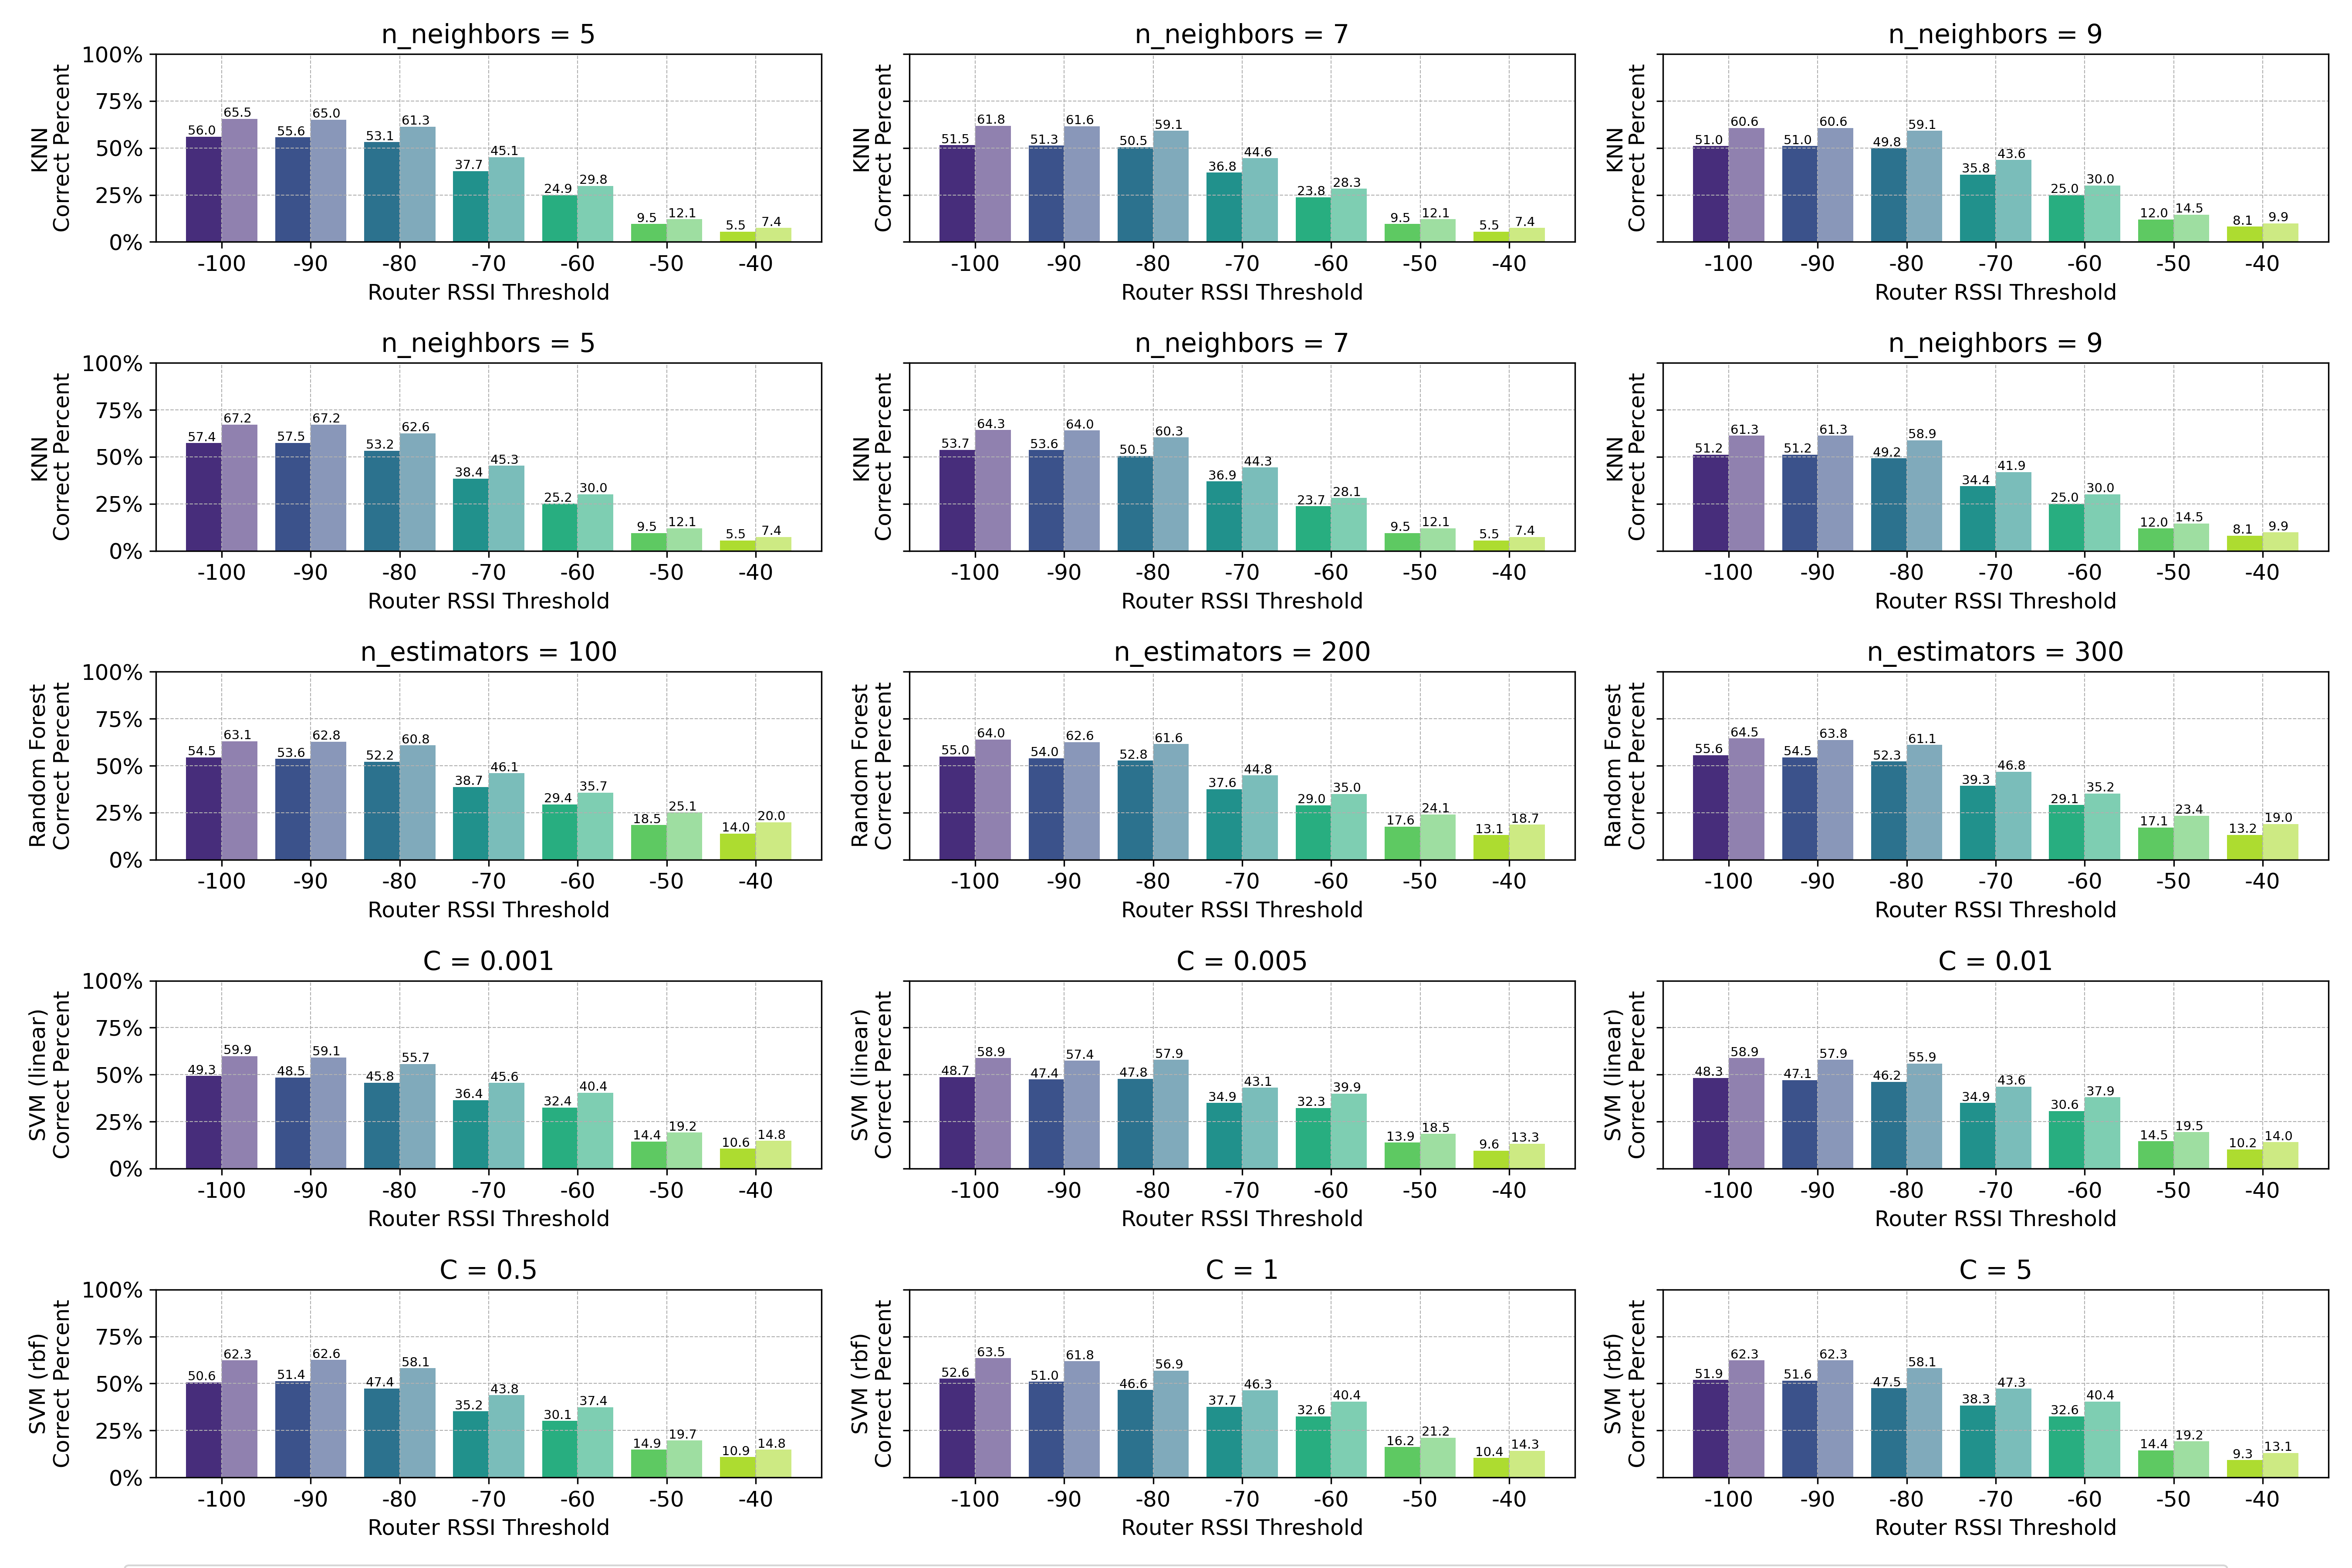
\includegraphics[width=0.8\textwidth]{images/6_router_rssi_threshold_01.png}
    \caption{Router Rssi Threshold}
    \label{fig:6_router_rssi_threshold_01}
\end{figure}

\section{Skalierung der RSSI-Werte}
\begin{itemize}
    \item \textbf{Skalierungsmethoden:} Beschreiben Sie die verschiedenen Skalierungsmethoden (exponentiell, power, linear).
    \item \textbf{Anwendung der Skalierung:} Erklären Sie, wie die Skalierung auf die RSSI-Werte angewendet wird.
    \item \textbf{Einfluss der Skalierung:} Diskutieren Sie den Einfluss der verschiedenen Skalierungsmethoden auf die Ergebnisse.
\end{itemize}

In Abbildung \ref{fig:value_scaling_strategies_ignore_10} sind die Ergebnisse der verschiedenen Strategien zur Auswahl der Value Scaling Strategy dargestellt.

\begin{figure}[H]
    \centering
    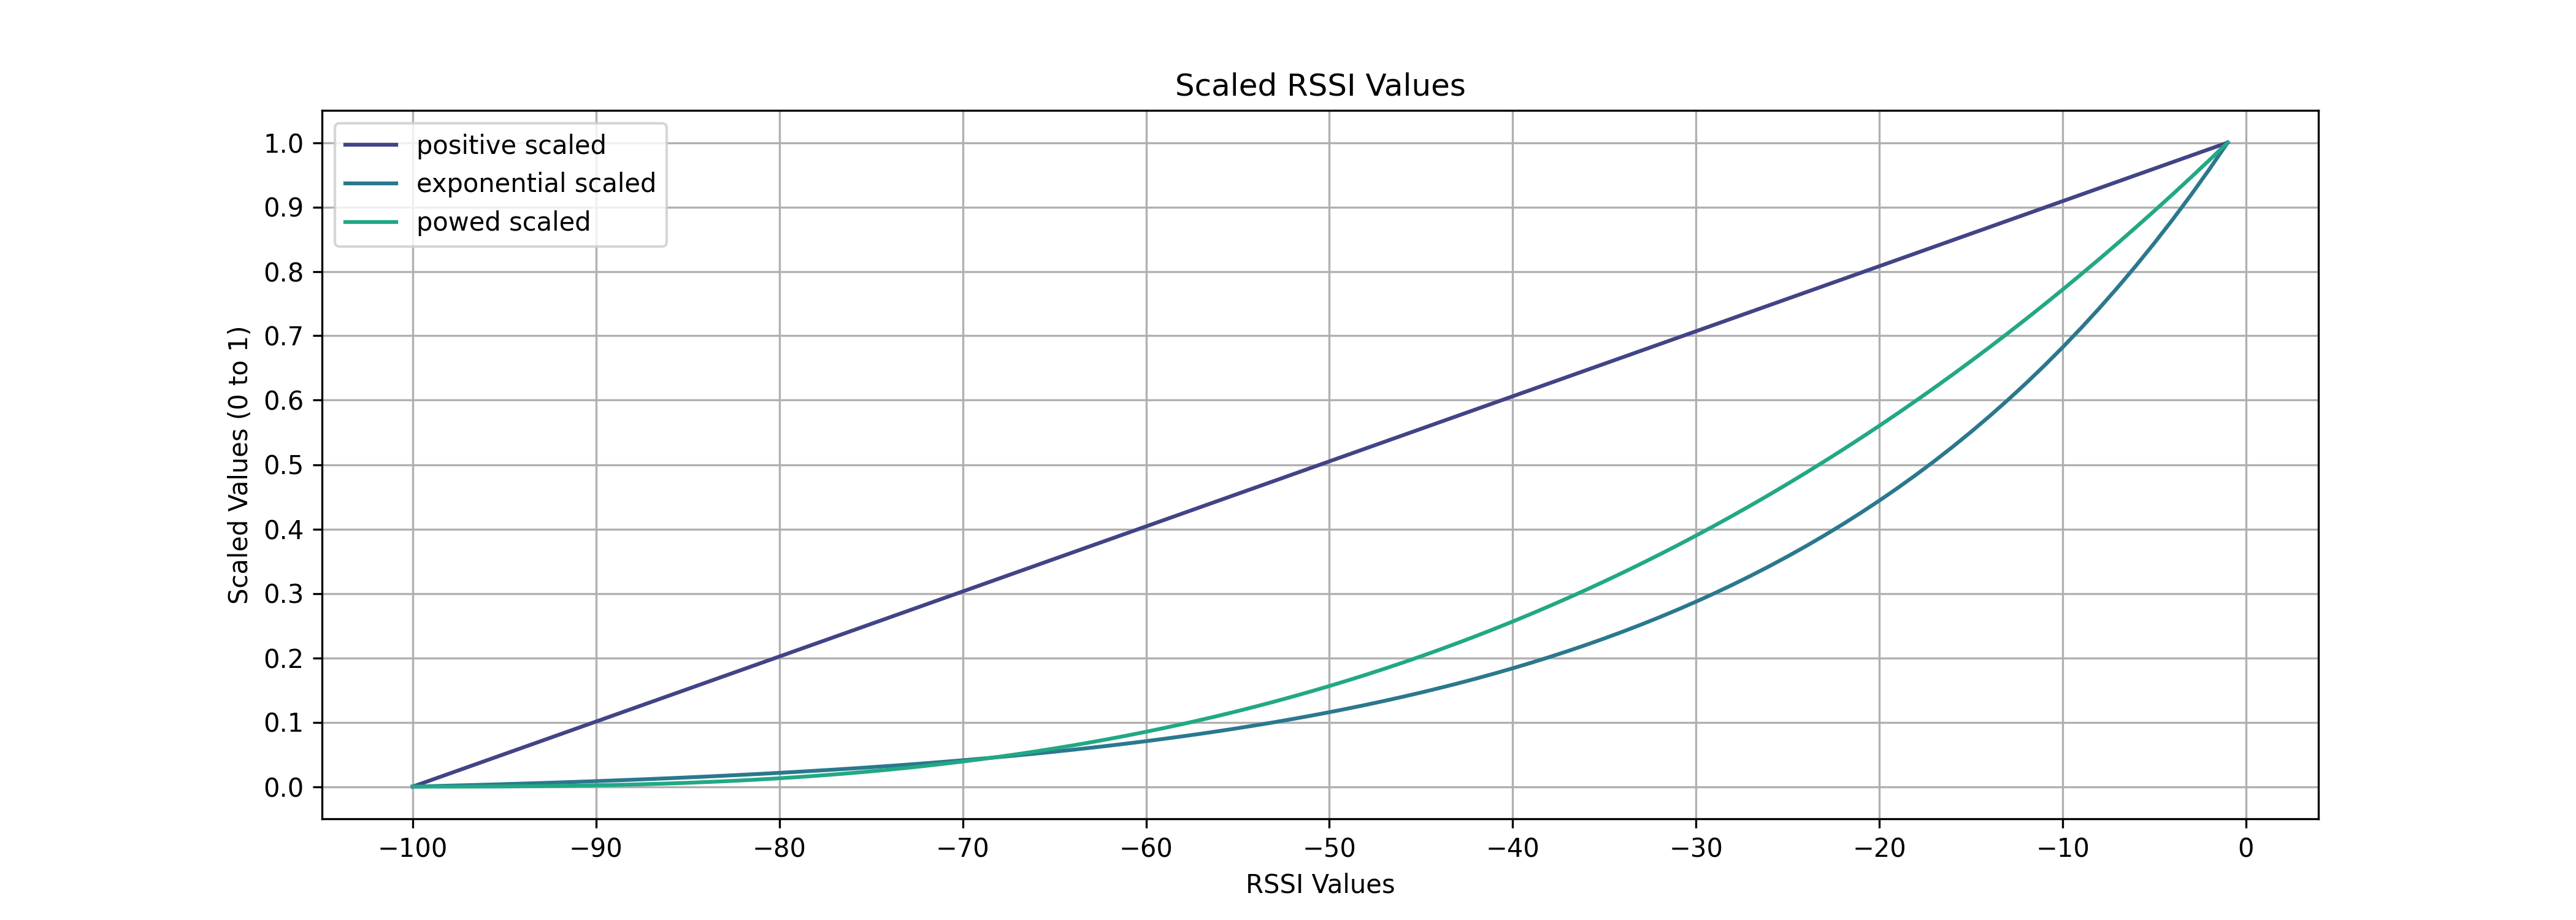
\includegraphics[width=0.8\textwidth]{images/value_scaling_strategies_ignore_10.png}
    \caption{Value Scaling Strategies}
    \label{fig:value_scaling_strategies_ignore_10}
\end{figure}

\subsubsection{Formeln}

Quelle: Comprehensive analysis of distance and similarity measures for Wi-Fi fingerprinting indoor positioning systems

Gegeben \(\alpha = 24\) und \(\beta = e\):

\subsection*{Positive Werte Repräsentation}
\begin{equation}
\text{Positiv}_i(x) = 
\begin{cases} 
\text{RSS}_i - \text{min} & \text{wenn WAP}_i vorhanden ist und \text{RSS}_i \geq \tau \\
0 & \text{andernfalls} 
\end{cases}
\end{equation}

\subsection*{Null-bis-Eins Normalisierte Werte}
\begin{equation}
\text{NullBisEinsNormalisiert}_i(x) = \frac{\text{Positiv}_i(x)}{-\text{min}}
\end{equation}

\subsection*{Exponentielle Repräsentation}
\begin{equation}
\text{Exponentiell}_i(x) = \frac{\exp\left(\frac{\text{Positiv}_i(x)}{\alpha}\right)}{\exp\left(\frac{-\text{min}}{\alpha}\right)}
\end{equation}

\subsection*{Potenzierte Repräsentation}
\begin{equation}
\text{Potenz}_i(x) = \left(\frac{\text{Positiv}_i(x)}{-\text{min}}\right)^{\beta}
\end{equation}

\subsection*{Werteskalierung}
Die Funktion zur Werteskalierung wendet die folgenden Transformationen basierend auf der gewählten Strategie an:

\textbf{Exponentielle Skalierung:}
\begin{equation}
X_{\text{skaliert}} = \text{Exponentiell}(X)
\end{equation}

\textbf{Potenzierte Skalierung:}
\begin{equation}
X_{\text{skaliert}} = \text{Potenz}(X)
\end{equation}

\textbf{Positive Skalierung:}
\begin{equation}
X_{\text{skaliert}} = \text{Positiv}(X)
\end{equation}

\textbf{Keine Skalierung:}
\begin{equation}
X_{\text{skaliert}} = X
\end{equation}

\subsubsection{Nochmal KNN Uniform vs. Distance}

Die Ergebnisse der verschiedenen Strategien zur Auswahl der Value Scaling Strategy sind in Abbildung \ref{fig:7_value_scaling_strategy_knn_distance_02} dargestellt.

\begin{figure}[H]
    \centering
    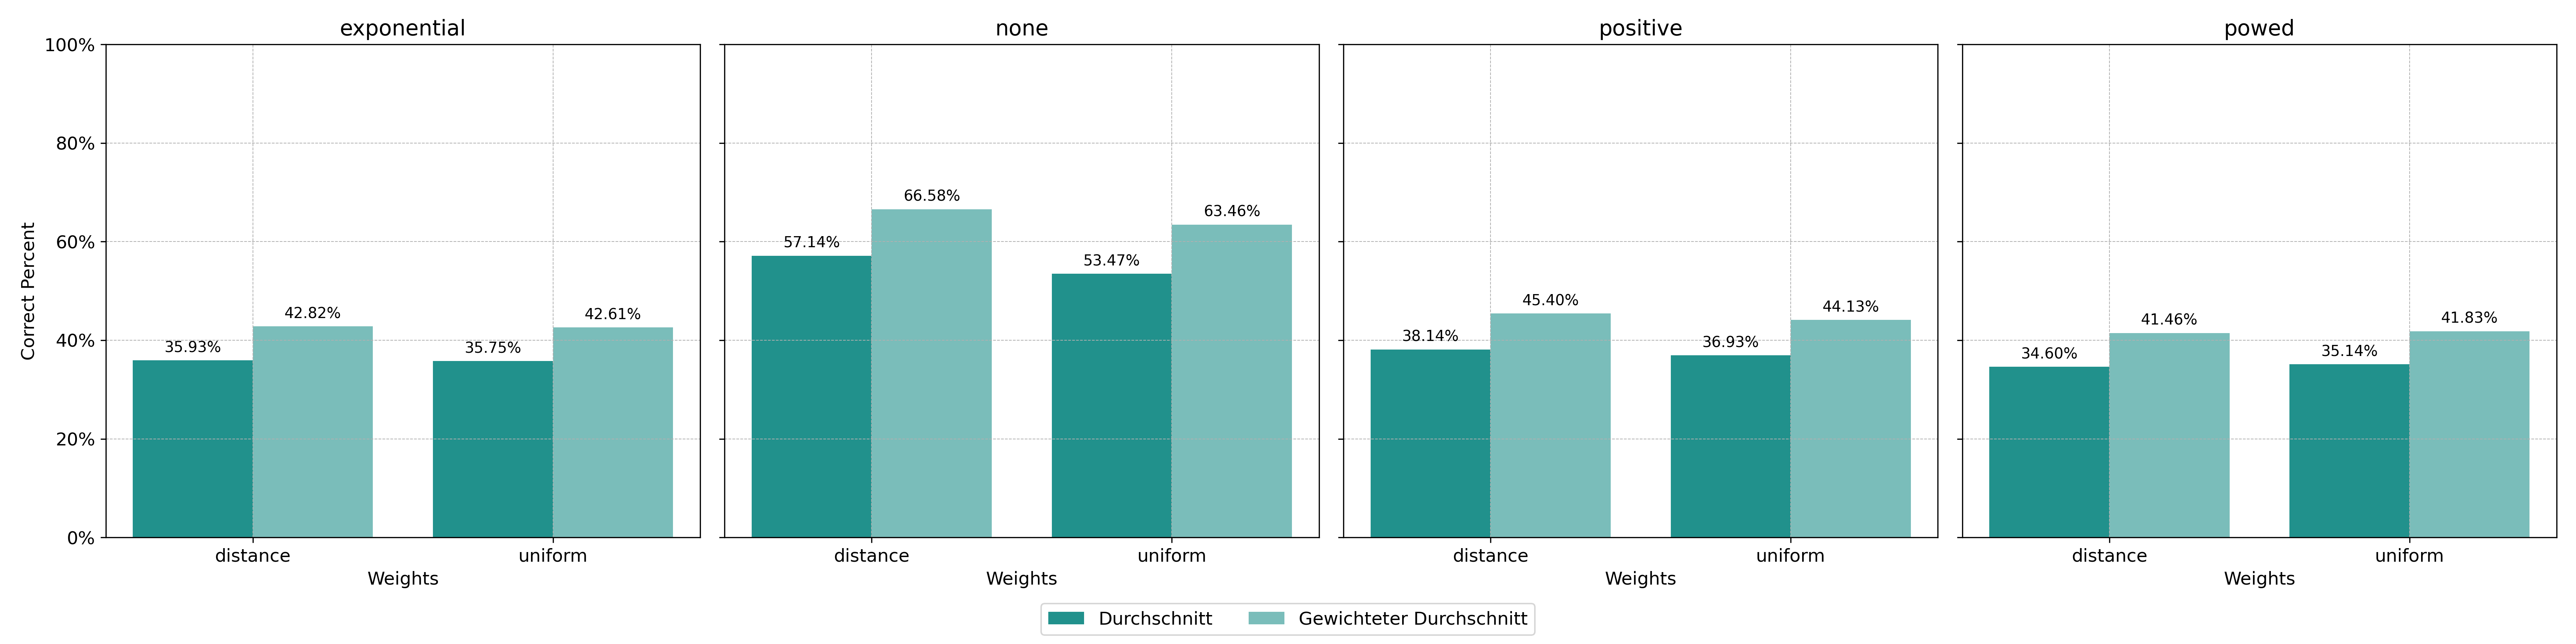
\includegraphics[width=0.8\textwidth]{images/7_value_scaling_strategy_knn_distance_02.png}
    \caption{Distance vs. Uniform}
    \label{fig:7_value_scaling_strategy_knn_distance_02}
\end{figure}

Die Ergebnisse der verschiedenen Strategien zur Auswahl der Value Scaling Strategy sind in Abbildung \ref{fig:7_value_scaling_strategy_knn_distance_03} dargestellt.

Das fällt auf in Abbildung \ref{fig:7_value_scaling_strategy_knn_distance_03}:
\begin{itemize}
    \item In den meisten fällen sehr ähnlicher Verlauf --> Es gibt Unterschiede bei den Skalierungsmethoden, aber bei den Skalierungsmethoden sind die Ergebnisse bei euclidean/sorensen und distance/uniform sehr ähnlich
    \item Bei exponential: distance ist besser als uniform bei wenigen Messungen pro Raum
    \item Bei none: distanz ist etwas besser als uniform bei wenigeren Messungen. Abstand nimmt aber ab mit der Anzahl an Messungen
    \item Bei exponential, powed (und auch leicht bei positive): Nimmt die Genauigkeit mit zunehmender Anzahl an Messungen wieder ab. Bisher hatten die Räume mit den meisten Messungen immer die größten Genauigkeiten. In diesem Fall haben die Räume mit 16 Messungen die höchste Genauigkeit und danach nimmt es wieder ab. Bei exponential und powed ist die Genauzigkeit bei n = 19 sogar wieder bei fast allen Kombinationen aus distance und weights bei 0\%!
\end{itemize}    

\begin{figure}[H]
    \centering
    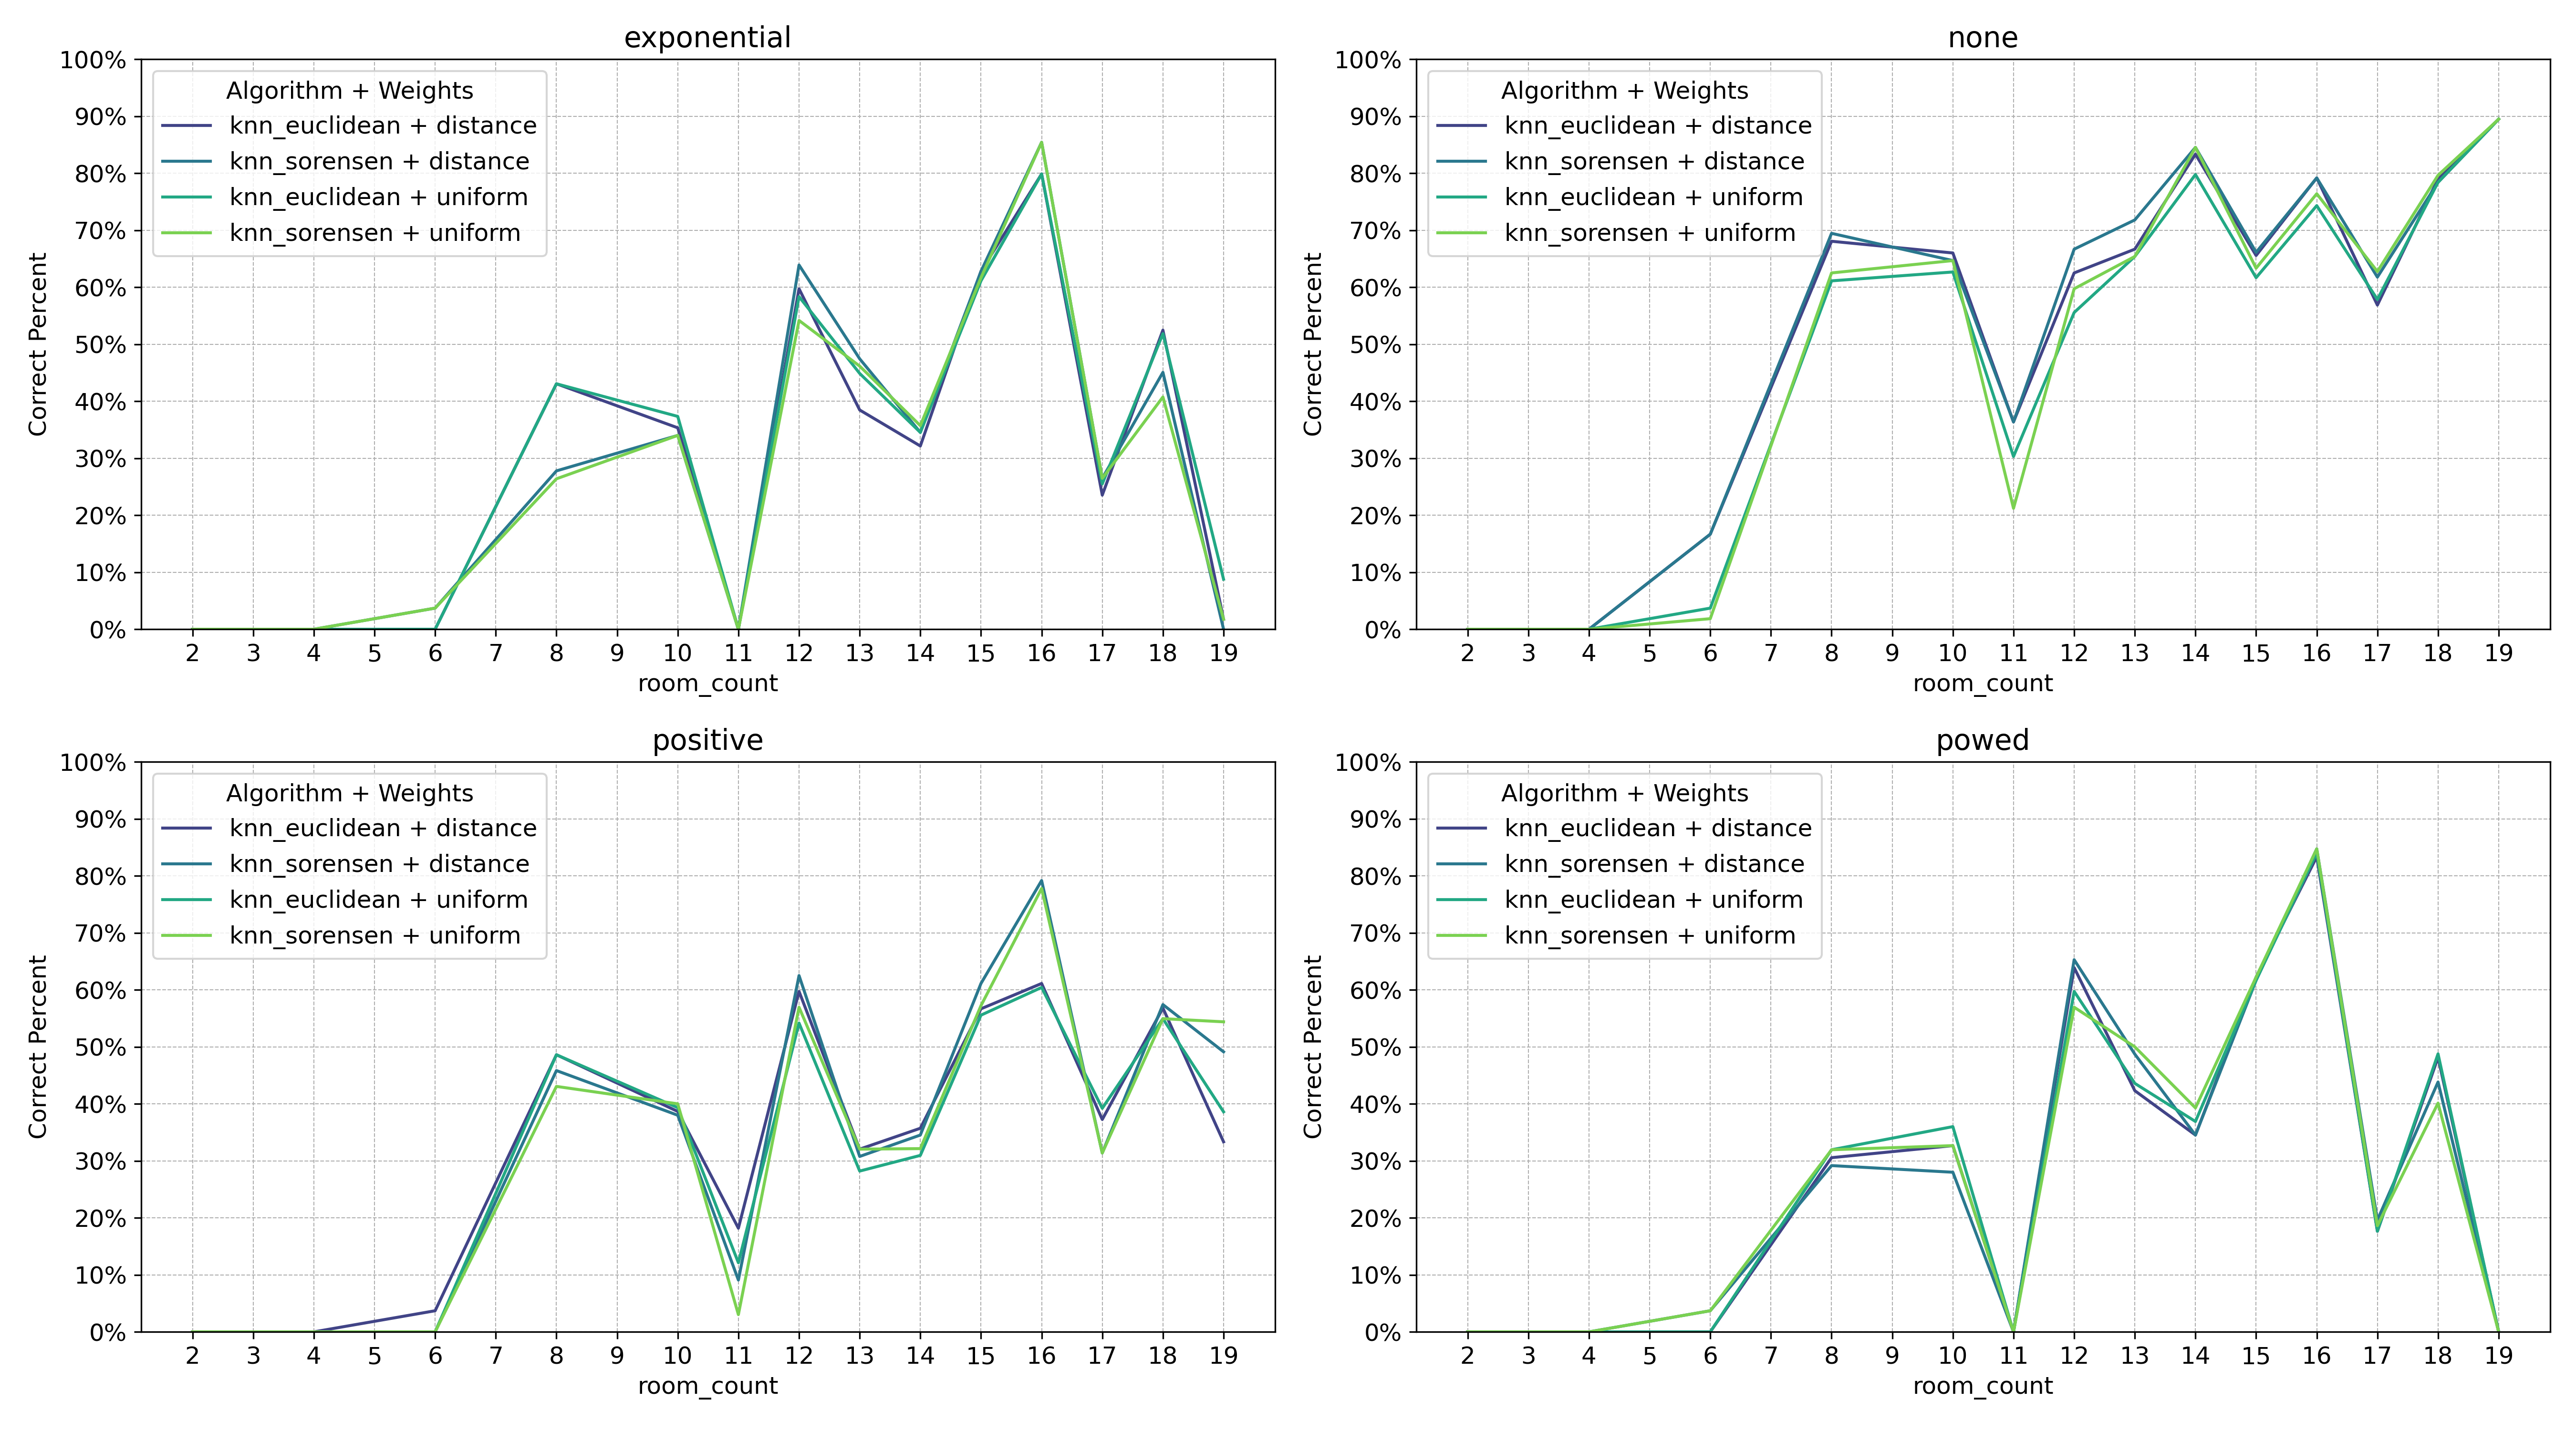
\includegraphics[width=0.8\textwidth]{images/7_value_scaling_strategy_knn_distance_03.png}
    \caption{Distance vs. Uniform}
    \label{fig:7_value_scaling_strategy_knn_distance_03}
\end{figure}



TODOs:

\begin{itemize}
    \item Plots zu den verschiedenen Value Scaling Strategies
    \item Referent zum Paper (Comprehensive analysis of distance and similarity measures for Wi-Fi fingerprinting indoor positioning systems)
\end{itemize}  
